\documentclass[10pt]{report}
\usepackage{graphicx}
\renewcommand{\textheight}{25cm}
\begin{document}
\title{\v{R}e\v{s}en\'i soustav line\'arn\'ich rovnic\\ Gaussovou elimina\v{c}n\'i metodou\\ dokumentace}
\author{Alexander Mansurov, 6.C}
\maketitle
\section{Grafick\'e rozhran\'i}
\paragraph{Popis}Grafick\'e rozhran\'i se skl\'ad\'a ze dvou komponent typu Label, jedn\'e komponenty typu SpinEdit, dvou tla\v{c}\'itek, a jednoho StringGridu.
\paragraph{~}Jedna komponenta typu Label nen\'i z po\v{c}\'atku vid\v{e}t a slou\v{z}\'i pro zobrazen\'i \v{r}e\v{s}en\'i soustavy a druh\'a konstantn\v{e} informuje u\v{z}ivatele o tom, \v{z}e vedle se nach\'azej\'ic\'i komponentou SpinEdit nastavujeme po\v{c}et nezn\'am\'ych soustavy.
Jedno z tla\v{c}\'itek slou\v{z}\'i pro zm\v{e}nu po\v{c}tu nezn\'am\'ych, druh\'e pro zah\'ajen\'i v\'ypo\v{c}tu. Samotn\'a matice se zad\'av\'a pomoc\'i komponenty StringGrid.
\paragraph{Postup}Nejprve pomoc\'i SpinEditu vybereme po\v{c}et nezn\'am\'ych a tla\v{c}\'itkem Prekresli nastav\'ime rozm\v{e}ry StringGridu. StringGrid dostane popisky bun\v{e}k a bude do n\v{e}j povoleno zapisovat. U\v{z}ivatel n\'asledn\v{e} zad\'av\'a koeficienty rovnic a jejich pravou stranu. Nakonec odstartuje v\'ypo\v{c}et p\v{r}\'islu\v{s}n\'ym tla\v{c}\'itkem a dostane v\'ysledek v p\v{r}\'islu\v{s}n\'em Labelu.\begin{center}
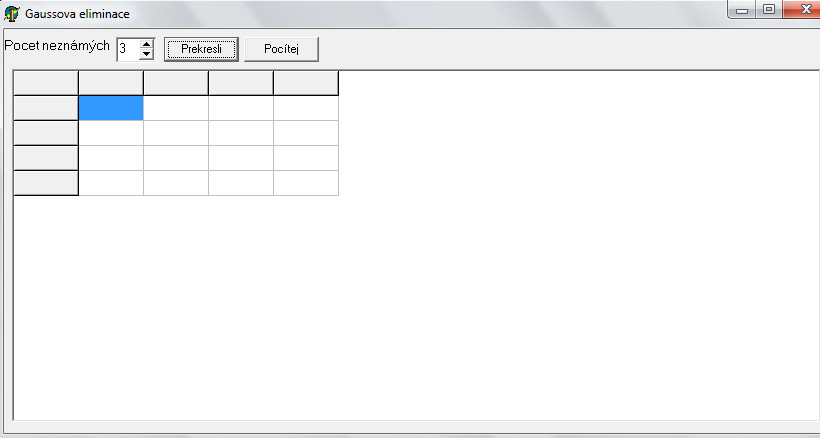
\includegraphics[width=10cm]{ge.jpg}
\end{center}
\section{Pohled pod pokli\v{c}ku}
\paragraph{TForm1.Button2Click (\v{r}\'adek 137)}Kdy\v{z} u\v{z}ivatel odstartuje v\'ypo\v{c}et, nejprve dojde k zaps\'an\'i vstupn\'ich dat do vnit\v{r}n\'ich datov\'ych struktur. V r\'amci programu se pou\v{z}\'ivaj\'i dva vlastn\'i datov\'e typy: Matrix a Vector. Matrix je dvojrozm\v{e}rn\'e pole re\'aln\'ych \v{c}\'isel velikosti 10x10, Vector jednorozm\v{e}rn\'e pole re\'aln\'ych \v{c}\'isel velikosti 10. Pole jsou indexovan\'a od 0 do 9. Koeficienty matice soustavy se ukl\'adaj\'i po sloupc\'ich do prom\v{e}nn\'e matice typu Matrix. Koeficienty prav\'e strany se ukl\'adaj\'i do prom\v{e}nn\'e vektor typu Vector. Tyto struktury spolu s \v{c}\'islem n ozna\v{c}uj\'ic\'im po\v{c}et nezn\'am\'ych se p\v{r}edaj\'i procedu\v{r}e gauss, prov\'ad\v{e}j\'ic\'i vlastn\'i eliminaci.
\paragraph{gauss (\v{r}\'adek 107)}Gaussova eliminace s v\'yb\v{e}rem pivota. Proch\'az\'ime matici po
 \v{r}\'adc\'ich. Pro ka\v{z}d\'y \v{r}\'adek nalezneme pivota - nejv\v{e}t\v{s}\'i prvek ve sloupci
  pod hlavn\'i diagon\'alou, tj. pro i-t\'y \v{r}\'adek, pod i-t\'ym sloupcem -  u\v{z}it\'im funkce
   pivot\_lookup. Pokud pivot nen\'i v matici na pozici [i,i], pomoc\'i procedury swap dojde k
    prohozen\'i \v{r}\'adk\r{u} v matici tak, aby se pivot posl\'eze nach\'azel na pozici [i,i].
 \paragraph{~}
     Proch\'az\'ime i-t\'y sloupec od pozice [i,i] dol\r{u} a v ka\v{z}d\'em \v{r}\'adku, za
      podm\'inky, \v{z}e pivot nen\'i nula, proch\'az\'ime od i-t\'eho sloupce doprava a od
       jednotliv\'ych prvk\r{u} matice i vektoru ode\v{c}\'it\'ame pod\'il prvku v dan\'em \v{r}\'adku
        pod pivotem ku pivotu n\'asoben\'y prvkem matice ve stejn\'em sloupci z i-t\'eho \v{r}\'adku.
        Z\'arove\v{n} od vektoru (prav\'e strany rovnice) ode\v{c}teme pod\'il prvku v dan\'em
         \v{r}\'adku pod pivotem ku pivotu n\'asoben\'y prvkem vektoru ve stejn\'em sloupci z i-t\'eho
          \v{r}\'adku.       
\paragraph{~} V p\v{r}\'ipad\v{e}, \v{z}e by
        pivot byl nula, nastane v\'yjimka o nedovolen\'em d\v{e}len\'i nulou a z\'arove\v{n}
         u\v{z} z funkce pivot\_lookup obdr\v{z}\'ime hl\'a\v{s}ku o nejednozna\v{c}nosti
          \v{r}e\v{s}en\'i. Pokud k chyb\v{e} nedojde, pust\'ime se do reverzn\'i substituce pomoc\'i procedury rev\_sbst.         
\paragraph{pivot\_lookup (\v{r}\'adek 44)} Funkce hled\'a nejv\v{e}t\v{s}\'i prvek v i-t\'em sloupci,
 vrac\'i \v{c}\'islo \v{r}\'adku tohoto prvku nebo nast\'av\'a v\'yjimka pokud by tento pivot byl rovn\'y
  nule, jeliko\v{z} by \v{r}e\v{s}en\'i soustavy nebylo jednozna\v{c}n\'e.
\paragraph{swap (\v{r}\'adek 76)} Procedura prohod\'i v i-t\'em sloupci matice k-t\'y prvek s prvkem
 ozna\v{c}en\'ym jako pivot a z\'arove\v{n} prohod\'i i-t\'y prvek vektoru s prvkem ozna\v{c}en\'ym
  jako pivot.
\paragraph{rev\_sbst (\v{r}\'adek 113)} Procedura kon\'a zp\v{e}tn\'y chod po kter\'em je ve vektoru
 \v{r}e\v{s}en\'i soustavy, pokud existuje, nebo nastane v\'yjimka o neexistenci \v{r}e\v{s}en\'i
  soustavy.
\paragraph{~}Pokud v prav\'em doln\'im rohu matice je nula a z\'arove\v{n} je posledn\'i prvek vektoru
 nula, pak se hod\'i v\'yjimka, \v{z}e soustava m\'a nekone\v{c}n\v{e} mnoho \v{r}e\v{s}en\'i, pokud v\v{s}ak posledn\'i prvek vektoru nen\'i nula, nastane v\'yjimka, \v{z}e
   soustava nem\'a \v{r}e\v{s}en\'i.
\paragraph{~}Do i-t\'e rovnice dosazujeme vypo\v{c}\'itan\'e hodnoty $x_i$ a\v{z} $x_n$, vyj\'ad\v{r}\'ime a vypo\v{c}\'it\'ame nezn\'amou $x_i$.
\subsection{Dal\v{s}\'i pomocn\'e procedury}
\paragraph{TForm1.Button1Click (\v{r}\'adek 65)} Nastav\'i velikost StringGridu na $n*(n+1)$, kde n je po\v{c}et rovnic zadan\'y u\v{z}ivatelem p\v{r}es komponentu SpinEdit.
\paragraph{outprint (\v{r}\'adek 149)} Vyp\'i\v{s}e mno\v{z}inu \v{r}e\v{s}en\'i na obrazovku do Labelu2
\paragraph{popis\_stringgrid (\v{r}\'adek 152)} P\v{r}id\'a popisky na kompnentu StringGrid pro u\v{z}ivatelskou p\v{r}\'iv\v{e}tivost
\end{document}